% Chapter - Player Study - Physical Health effects
\chapter{Physical Health Effects}
\label{chapter:player-study-physical}
\lhead{Chapter \ref{chapter:player-study-physical}. \emph{Player Study - Physical Health Effects}}

This chapter examines the survey results in the context of determining th game's effect on the physical health of its players. The questions in Table \ref{tbl:rg2-survey-questions} and their answers are the main focus of this chapter, but relevant answers to other questions are also included.

\section{Results for Change in Physical Activity}

This section presents the results for the player survey questions related to Research Questions \ref{RQ2.1}, \ref{RQ2.2} and \ref{RQ2.3}. A total of 2193 subjects responded to the questions \emph{"In an average week, how much time did you spend on physical activities (e.g. walking, running or biking) before you started playing Pokémon Go?"} and \emph{"In an average week, how much time do you spend on physical activities since you started playing Pokémon Go?"}. Table \ref{tbl:physical-activity-before-and-after} shows the number of responses to each question (column 2 and 3 respectively), as well as the change \todo{(should it say delta?)}, within each time category. Percentages for the \emph{Before} and \emph{After} columns are the percentage of total respondents for the respective category, while the percentage in the \emph{Change} column shows the relative increase or decrease (negative percentages) for that category. Note that the percentages are rounded to the closest integer, and due to rounding errors, the percentages in column 2 and 3 sum to 101 \% and 99 \% respectively.

\begin{table}[h]
	\centering
	\caption{Physical activity before and after Pokémon GO}
	\label{tbl:physical-activity-before-and-after}
	\begin{tabular}{|l|c|c|c|}
		\hline
		\textbf{Hours of activity} & \textbf{Before} & \textbf{After} & \textbf{Change} \\\hline\hline
		30 minutes or less	& 395 & 32 & -363\\
							& 18\% & 1\% & -92\%\\\hline
		An hour or less & 324 & 107 & -217\\
						& 15\% & 5\% & -67\%\\\hline
		2 hours or less & 384 & 268 & -116\\
						& 18\% & 12\% & -30\%\\\hline
		4 hours or less & 477 & 515 & 38\\
						& 22\% & 23\% & 8\%\\\hline
		8 hours or less & 394 & 566 & 172\\
						& 18\% & 26\% & 44\%\\\hline
		12 hours or less	& 132 & 365 & 233\\
							& 6\% & 17\% & 177\%\\\hline
		20 hours or less	& 61 & 206 & 145\\
							& 3\% & 9\% & 238\%\\\hline
		More than 20 hours	& 26 & 134 & 108\\
							& 1\% & 6\% & 415\%\\\hline
	\end{tabular}
\end{table}

Respondents were also asked what activities lead to the increase in their physical activity, if they had become more physically active. Table \ref{tbl:physical-activity-sources} shows the number of respondents for each activity out of 1828 respondents who had an increase in physical activity.

\begin{table}[h]
	\centering
	\caption{Reasons for increased physical activity from Pokémon GO}
	\label{tbl:physical-activity-sources}
	\begin{tabular}{|c|c|c|c|}
		\hline
		\textbf{Detours} & \textbf{Errands} & \textbf{Pokéhunting} & \textbf{Other}\\\hline\hline
		1136 & 636 & 1576 & 99\\
		62\% & 35\% & 86\% & 5\%\\\hline
	\end{tabular}
\end{table}

\todo{Explain activities here, mention some "Other" activities, and people who reported N/A etc}

\section{Analysis of Results for Change in Physical Activity}

\begin{figure}[h]
	\centering
	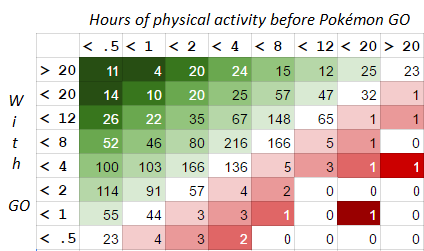
\includegraphics{Figures/change-in-physical-activity-table-colors}
	\caption{Change in physical activity with Pokémon GO}
\end{figure}

\section{Benefits}

\todo{Increased physical activity, weight loss and general feeling of wellness, skipping unhealthy activities}

\section{Neglect and Negative Behavior}


% Chapter
\chapter{Mental Health Effects}
\label{chapter:player-study-mental}
\lhead{Chapter \ref{chapter:player-study-mental}. \emph{Player Study - Mental Health Effects}}

\todo{Maybe combine the following into just two sections - negative and positive}

\section{Social Interaction}
\label{sub:mental-health-social}

\todo{Mention division of tasks (searching for nearby pokes, scoping out gyms, and transporter/player), and that players on different teams still can cooperate and be on good terms}

\section{Exercise}

\section{A Sense of Purpose}

\section{Disappointment}

\section{Negative Behavior and Adversarial Relationships}